\documentclass{article}

%opening
\title{Manco il titolo mi ricordo}
\author{Cristina Caprioglio}
\date{2023/2024 }
\usepackage[margin=0.75in]{geometry}
	\usepackage{amssymb}
	\usepackage{amsmath}
	\usepackage{multicol}
	\usepackage{graphicx}
	\usepackage{physics}
	\usepackage{subcaption}
	\usepackage{float}
	\usepackage[justification=centering]{caption}
\begin{document}

\maketitle

\section*{Introduction}
Galaxy clusters are the largest collapsed structures in the Universe, with the most regular ones being almost virialised and with $M_{vir}\gtrsim 10^{14}$ M$_{\odot}$ and $R_{vir}\gtrsim 1$ Mpc. They are gravitationally bound aggregations of galaxies containing from $\sim 50$ up to a few $10^{3}$ galaxies., with most of their mass in the form of dark matter, with $\sim 10-16\%$ of their mass in the form of baryons, mostly hot gas ($T\sim 10^{7\text{\textemdash}8}$ K) called the intracluster medium (ICM). This diffuse ($n\sim 10^{-1}\text{\textendash}10^{-3}$ cm$^{-3}$) is a fully ionized plasma which is weakly collisional and it's almost hydrostatic, supported by thermal pressure (while the galaxies are supported by the dynamical one). 
Its interaction with the galaxies is a key process in modern astrophysics.
Stars are also present,but they make only $1\text{\textendash}5\%$ of the total mass of the cluster. Many clusters host in their centre a large elliptical galaxy, with a mass of $\sim 5\times 10^{11\text{\textemdash}12}$ M$_{\odot}$ (the most massive ones can get up to $10^{13}$ m$_{\odot}$) and a massive black hole at the centre, which provides a huge amount of energy to the ICM (aka the AGN feedback). These galaxies are called \textit{brightest cluster galaxies} (or BCGs for short), and aside from being the most luminous in the cluster they play a key role in its evolution.
\\For a more detailed discussion on galaxy clusters, please refers to \cite[Sec. 6.4]{cimatti}.\\
We wanted to understand what could be the cause behind the outward iron spreading through the ICM. In order to do that, we divide the project in two parts: first, we model numerically the hydrostatic equilibrium of the hot gas in the cluster potential well, then we proceed to model the time evolution of the Fe abundance profile. We chose as a model the Perseus cluster and we followed the work by Rebusco et al. (2005)\cite{rebusco}.\\
We developed the numerical code using Fortran90, while for the plots we used gnuplot. 
\section{Hydrostatic configuration}
\subsection{Physical model}
The first part of the project is about understanding how the gas is distributed in a cluster, and to do so a proper gravitational model is needed.
We'll assume spherical symmetry, which will lead to all physical quantities depending only on $r$, the radial coordinate, which indicates the distance from the centre of the system.
The gas is supported by thermal pressure and it's described by the hydrostatic equilibrium equation:
\begin{equation}\label{idro_eq}
	\derivative{P}{r}=-\frac{GM(<r)}{r^{2}}\rho_{g}(r),
\end{equation}
which is a I order ODE. We have that in \eqref{idro_eq} $M(<r)$ indicates the total mass contained in a radius $r$, not just the mass of the gas, while $P$ and $\rho_{g}$ refer to the pressure and the density of the gas. \\
We have that the ICM is in equilibrium in the gravitational potential of the cluster, which is dominated by dark matter. \\
For the density profile of the latter we will assume a $Navarro-Frenk-White$ (NFW) $profile$, which takes the following form:
\begin{equation}\label{NFW}
	\rho_{DM}(r)=\frac{\rho_{DM,0}}{\left(\frac{r}{r_{s}}\right)\left(1+\frac{r}{r_{s}}\right)^{2}},
\end{equation}
where $\rho_{DM,0}$ and $r_{s}$ are parameters which depend on the cluster mass. 
Integrating \eqref{NFW} we can calculate the mass profile, which as an analytical solution:
\begin{equation}\label{massDM}
	M_{DM}(r)=\int_{0}^{r}4\pi r'^{2}\rho_{DM}(r')\dd{r'}=4\pi\rho_{DM,0}r_{s}^{3}\left[\ln\left(1+\frac{r}{r_{s}}\right)-\frac{r/r_{s}}{1+r/r_{s}}\right].
\end{equation}
To have a more realistic model we will also need to consider the presence of the BCG. Its stellar mass is described by the $Hernquist\; profile$:
\begin{equation}\label{Hern}
	M_{*}(r)=M_{BCG}\frac{r^{2}}{(r+a)^{2}},
\end{equation}
where $M_{BCG}$ is the mass of the elliptical central galaxy and $a$ is a scale related to the half-mass radius $r_{1/2}$: $r_{1/2}=(1+\sqrt{2})a$.\\
Assuming the ICM is described by the perfect gas equation of state (i.e. $P=\frac{k_{B}\rho_{g}T_{g}}{\mu m_{p}}$), \eqref{idro_eq} becomes:
\begin{equation}\label{hydroperf}
	\derivative{\ln \rho_{g}}{r}=-\frac{GM(<r)}{r^{2}}\frac{\mu m_{p}}{k_{B}T_{g}(r)}-\derivative{\ln T_{g}}{r},
\end{equation}
where $T_{g}(r)$ is the gas temperature, while $\mu ,\, m_{p},$ and $k_{B}$ are constants that represent the mean molecular weight, the proton mass and the Boltzmann constant respectively.\\
In the case of an isothermal gas and in the absence of the BCG eq.\eqref{hydroperf} has an analytical solution:
%\begin{equation}
	\begin{gather}\label{isogas}
		\rho_{g}=\rho_{0}\exp\left\{-\frac{27}{2}b\left[1-\frac{\ln (1+r/r_{s})}{r/r_{s}}\right]\right\}=\rho_{0}e^{-27b/2}\left(1+\frac{r}{r_{s}}\right)^{27b/(2r/r_{s})},\\
	with \quad b=\frac{8\pi G\mu m_{p}\rho_{DM,0}r_{s}^{2}}{27k_{B}T_{g,iso}}\notag
	\end{gather}
%\end{equation}
\subsection{The simulation}
The first step is building two uniform grids, with one shifted by $\frac{1}{2}\Delta r$, where $\Delta r=r\textsubscript{j}-r\textsubscript{j-1}$. The maximum number of points in the grids is $j\textsubscript{max}=5000$, while $r$ ranges from $r\textsubscript{min}=0 Mpc$ to $r\textsubscript{max}=3 Mpc$.
The points for the first grid are going to be
\begin{equation}
	r_{j}=r_{min}+\frac{j-1}{j_{max}-1}r_{max},\qquad 1\le j\le j_{max}
\end{equation}
so we'll use integer numbers to refer to them, while we'll use half-integers for the points in the second one.
We'll thus need to define not only the points but also $r_{jmax+1/2}$, which we'll do as follows:
\begin{equation}
	\begin{cases}
		r_{jmax+1/2}=r\textsubscript{jmax-1/2}+(r\textsubscript{jmax-1/2}-r\textsubscript{jmax-3/2})\\
		r\textsubscript{j+1/2}=r\textsubscript{j}+\frac{r\textsubscript{j+1}-r\textsubscript{j}}{2} \qquad 1\le j\le j_{max}-1
	\end{cases}
\end{equation}
Both the temperature $T$ and the density $\rho$ are centered at $r\textsubscript{j+1/2}$, while we centered the mass to $r\textsubscript{j}$.\\
To proceed with the simulation, we first integrate numerically $\rho\textsubscript{DM}$ in order to get $M\textsubscript{DM}$.
Assuming $ M\textsubscript{DM,1}=0$, we get the following expression:
\begin{equation}
	M\textsubscript{DM,j}=M\textsubscript{DM,j-1}+\rho\textsubscript{DM,j-1/2}\Delta V\textsubscript{j},
\end{equation}
where the j-th volume element $\Delta V\textsubscript{j}$ is given by:
\begin{equation}
	\Delta V\textsubscript{j}=\frac{4}{3}\pi(r^{3}_{j}-r^{3}_{j-1}).
\end{equation}
To check the integration we overplotted the results against the analytical solution found in \eqref{massDM}.\\
Once obtained $M_{DM}$ we can move on to the integration of \eqref{hydroperf}. We consider three possible scenarios:
\begin{itemize}
	\item isothermal gas without the presence of the BCG, where we have $\derivative{\ln T_{g}}{r}=0$ and $M_{j}=M_{DM,j}$;
	\item isothermal gas with the presence of the BCG, where we have $\derivative{\ln T_{g}}{r}=0$ and $M_{j}=M_{DM,j}+M_{*,j}$;
	\item non-isothermal gas with the presence of the BCG, where we have $\derivative{\ln T_{g}}{r}\ne 0$ and $M_{j}=M_{DM,j}+M_{*,j}$;
\end{itemize}
We transform \eqref{hydroperf} from an ODE to a FDE (finite difference equation), with the derivative centered in $j$:
\begin{equation}\label{11}
	\frac{\ln \rho_{g,j+1/2}-\ln \rho_{g,j-1/2}}{r_{j+1/2}-r_{j-1/2}}=-\frac{\mu m_{p}}{k_{B}\overline{T}_{g,j}}\frac{GM_{j}}{r_{j}^{2}}-\frac{\ln T_{g,j+1/2}-\ln T_{g,j-1/2}}{r_{j+1/2}-r_{j-1/2}},
\end{equation}
where $\overline{T}_{g,j}$ is defined as $\frac{T_{g,j+1/2}-T_{g,j-1/2}}{2}$. The expression for $\ln \rho_{g,j+1/2}$ can then be easily found from \eqref{11}:
\begin{equation} \label{numrho}
	\ln\rho_{g,j+1/2}=\ln\rho_{g,j-1/2}-\Delta r\frac{\mu m_{p}}{k_{B}\overline{T}_{g,j}}\frac{GM_{j}}{r_{j}^{2}}-(\ln T_{g,j+1/2}-\ln T_{g,j-1/2}).
\end{equation}
To find the appropriate values for the initial condition of the gas density we first run the code with an initial guess with the expected order of magnitude, then we adjust rthe values in order
to obtain a baryon fraction $f_{b}=\frac{M_{*}+M_{gas}}{M_{*}+M_{gas}+M_{DM}}$ close to the cosmic value ($\sim 0.16$) at the virial radius of the cluster ($r_{vir}\approx 2.8$ Mpc).\\
To conclude the setting of the simulations, the following list contains the parameters value and the temperature profiles:
\begin{itemize}
	\item for the NFW profile: $\rho_{DM,0}=7.35\times 10^{-26}$ g/cm$^{3}$ and $r_{s}=435.7$ kpc;
	\item for the $Hernquist$ $ profile$: $M_{BCG}=10^{12} M_{\odot}$ and $r_{1/2}=12$kpc;
	\item the initial condition $\rho_{g,0}$ for the gas density and the respective $f_{b}$ are: \begin{itemize}
		\item $4.1\times 10^{-26}$g/cm$^{3}$ and $0.159$ for the first scenario;
		\item $8\times 10^{-26}$g/cm$^{3}$ and $0.159$ for the second;
		\item $1.5\times 10^{-25}$g/cm$^{3}$ and $0.160$ for the third;
	\end{itemize}
	\item for both temperature pofiles we have $\mu=0.61$, while their expressions are:
	\begin{itemize}
		\item for the isothermal case: $T_{g}=T_{mg}=8.9\times 10^{7}$K;
		\item for the non-isothermal one:
		\begin{equation}\label{Tprof}
			\frac{T_{g}}{T_{mg}}=1.35\frac{(x/0.045)^{1.9}+0.45}{(x/0.045)^{1.9}+1}\frac{1}{(1+(x/0.6)^{2})^{0.45}}
		\end{equation}
		where $x=r/r_{500}$, with $r_{500}\sim r_{vir}/2=1.4$Mpc.
	\end{itemize}
\end{itemize}


\subsection{Results and discussion}
First we compare the analytical NFW mass profile to the numerical one, as well as to the Hernquist mass profile. These are plotted in Fig.\ref{fig:massprofiles}, and we can see how the analytical and numerical mass profile for dark matter barely differ, with a separation only noticeable in the first $2$ kpc.
\begin{figure}[H]
	
	\begin{subfigure}{0.49\textwidth}
		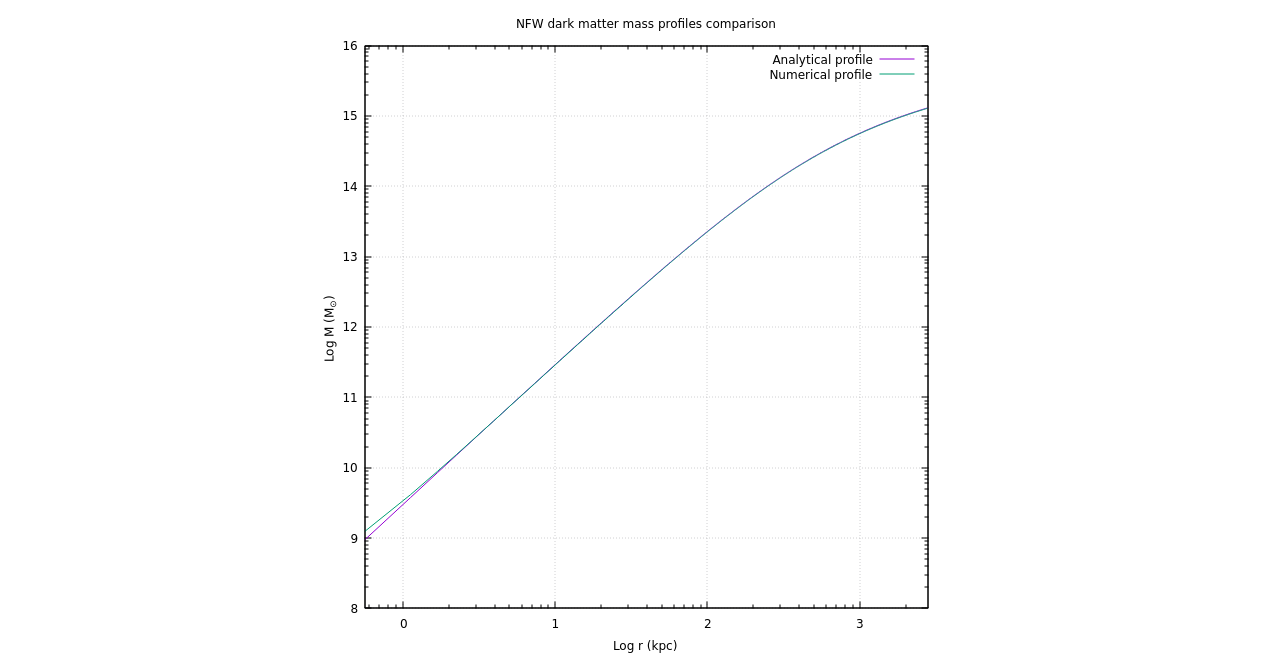
\includegraphics[width=0.9\linewidth]{dm_mass_profile.png}
	\end{subfigure}
	\begin{subfigure}{0.49\textwidth}
		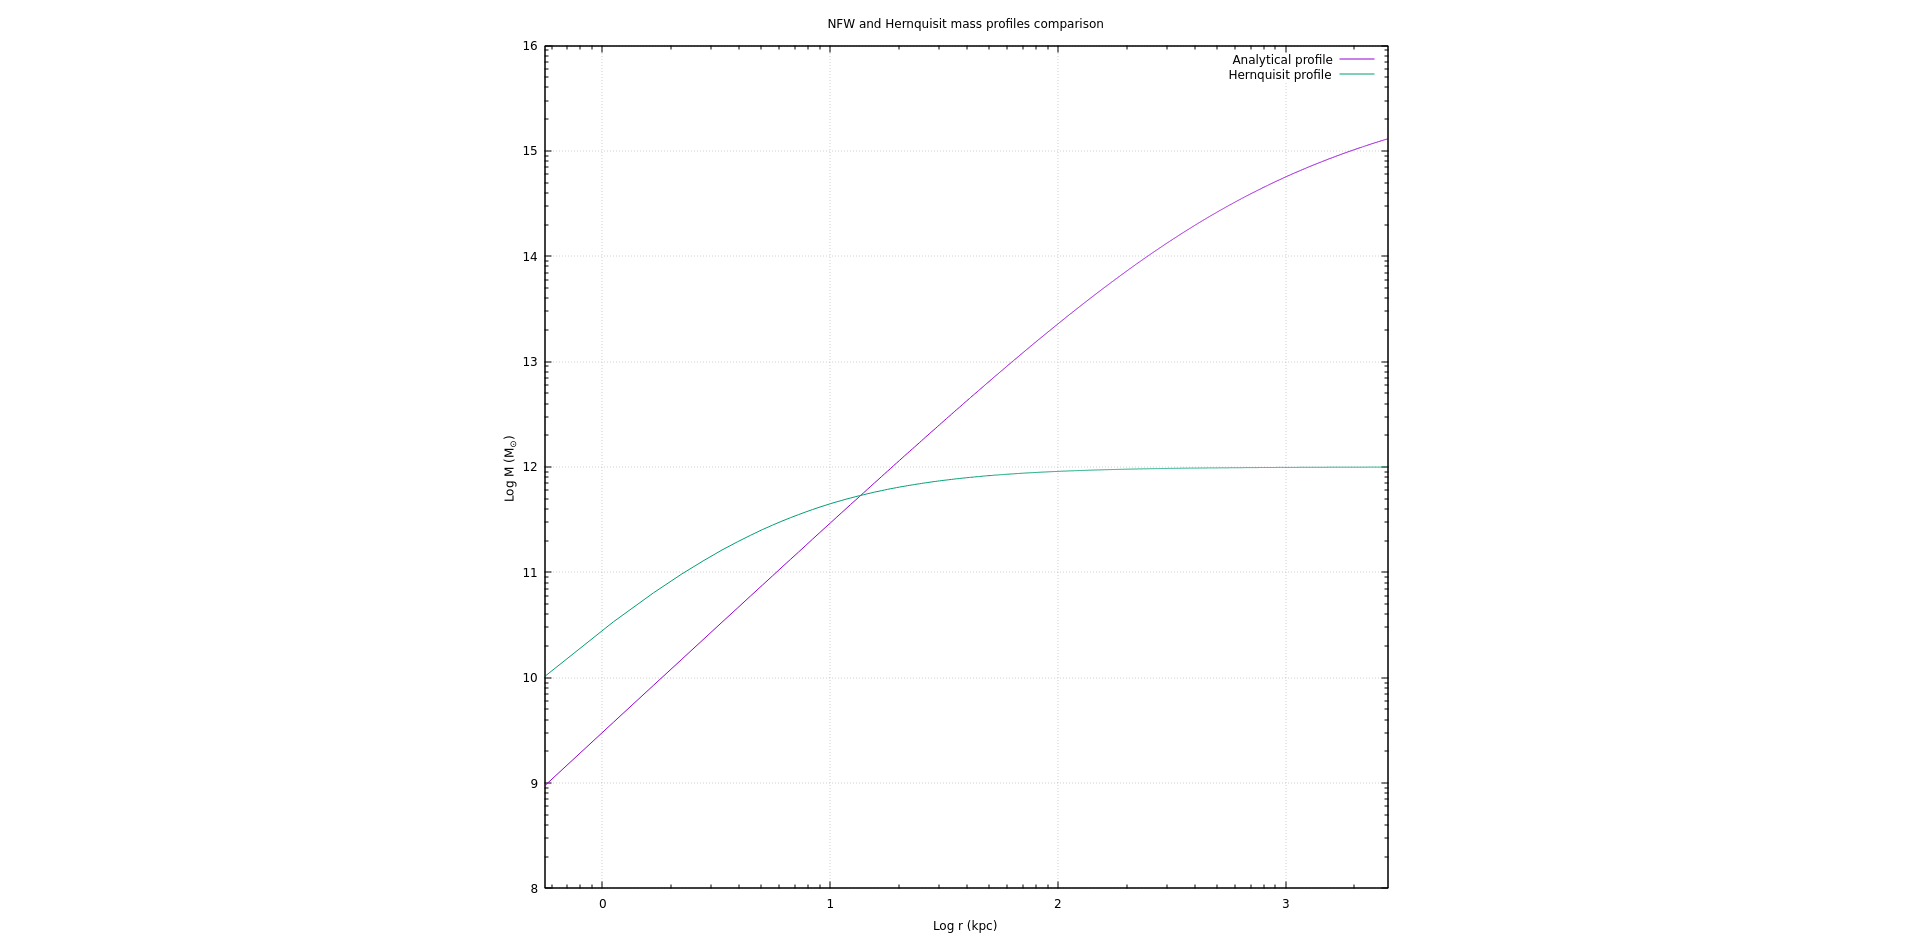
\includegraphics[width=0.9\linewidth]{mass_profiles.png}
	\end{subfigure}
	\centering
	\caption{On the left: analytical (purple curve) and numerical (green curve) NFW profiles. \\On the right: analitycal NFW (purple curve) and Hernquist (green curve) mass profiles.}
	\label{fig:massprofiles}
\end{figure}
In Fig.\ref{fig:densityprofiles} we plot the different density profiles, obtained through the numerical integration of \eqref{hydroperf} through \eqref{numrho}. \\
Comparing the isothermal models, we can notice how the presence of the BCG causes a steepening of the density profile in the
central regions. This is because of the term $\frac{GM(r)}{r^{2}}$ present in \eqref{hydroperf}, which represents the gravitational field, which increases with the presence of the BCG.
This is also the reason why you need to increase $\rho_{0}$ in order to keep the baryon fraction at $0.16$.\\
As for the differences between the isothermal model and the one with the temperature gradient, before we comment on the differences it's better to show the different temperature profiles, which is done in Fig.\ref{fig:tempprof}.
\begin{figure}[H]
	\centering
	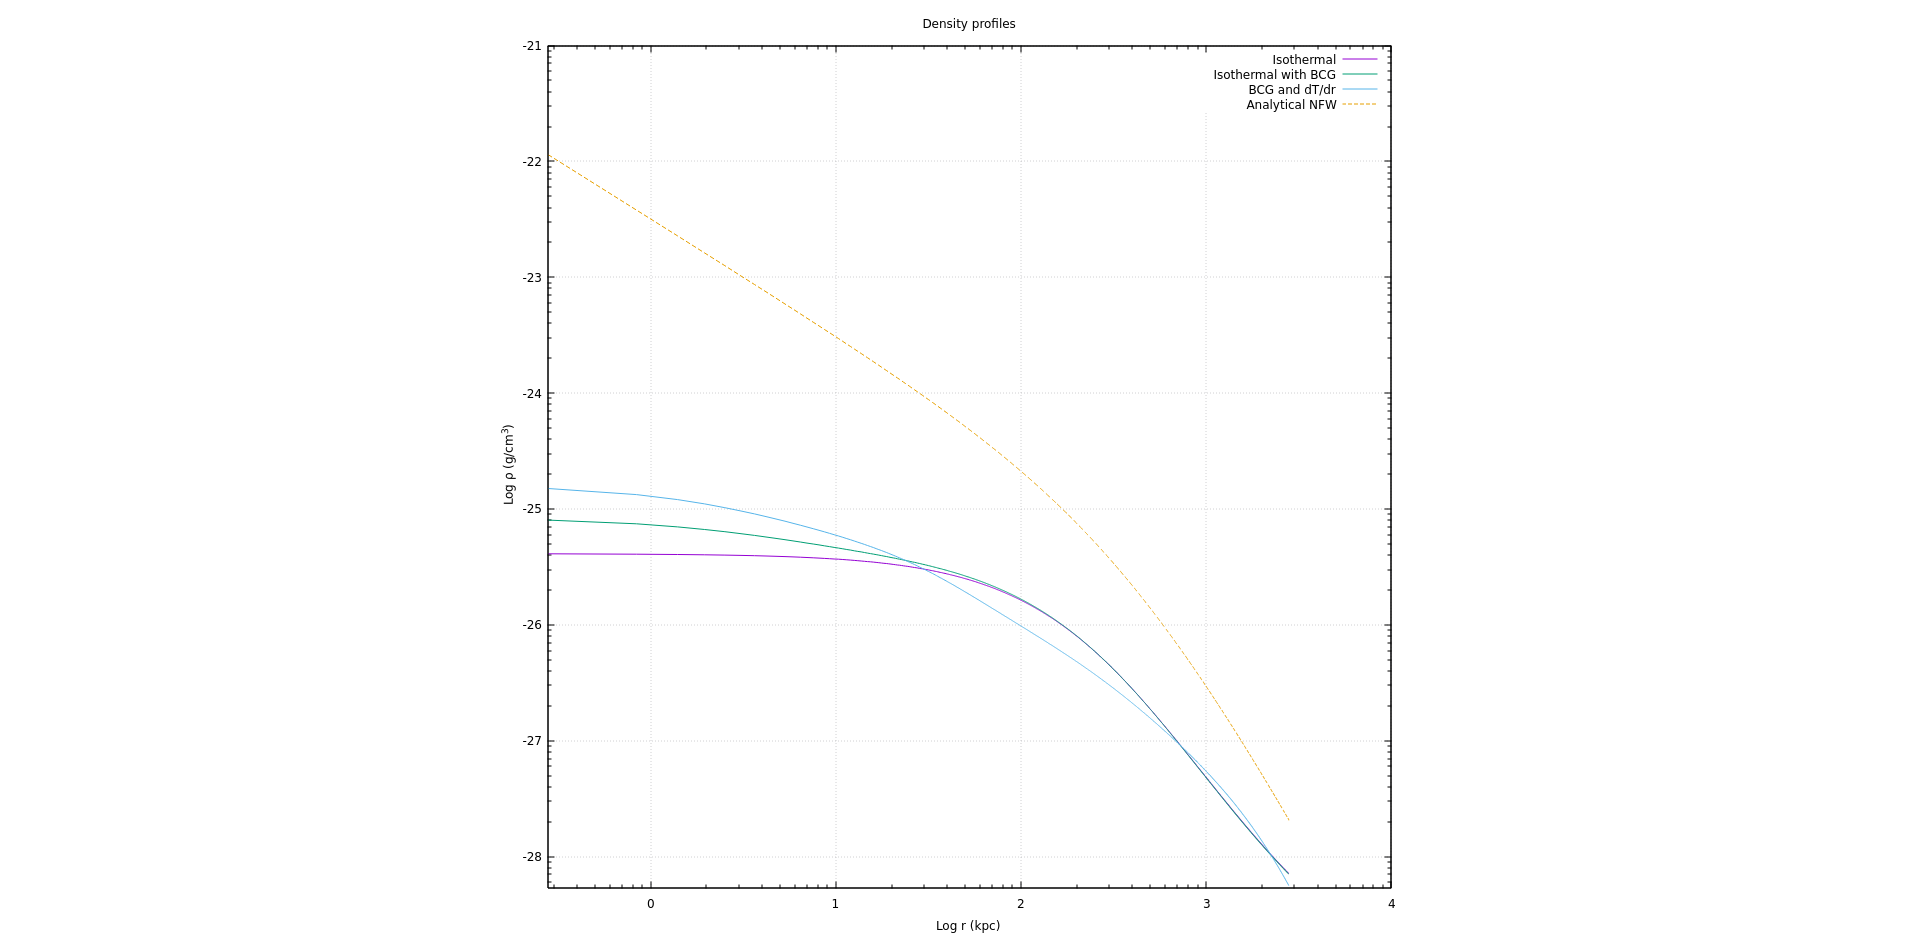
\includegraphics[width=\textwidth]{density_profiles.png}
	\caption{The different density profiles obtained from \eqref{hydroperf} for the following models: with only dark matter and isothermal gas (purple curve), with also the BCG but still isothermal (green curve), and with BCG and temperature gradient (light blue curve). 
	The analytical NFW profile for dark matter (dashed orange curve) is also plotted.}
	\label{fig:densityprofiles}
\end{figure}
\begin{figure}[H]
	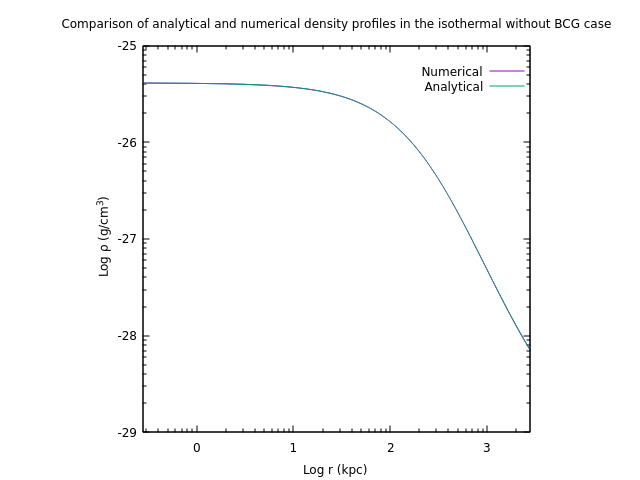
\includegraphics[width=\textwidth]{rhoiso.png}
	\caption{Comparison between the density profile obtained numerically for the isothermal model without the BCG (purple curve) and the analytical one given by \eqref{isogas} (green curve)}
	\label{fig:analvsnum}
\end{figure}
\begin{figure}[H]
	\begin{subfigure}{0.49\textwidth}
		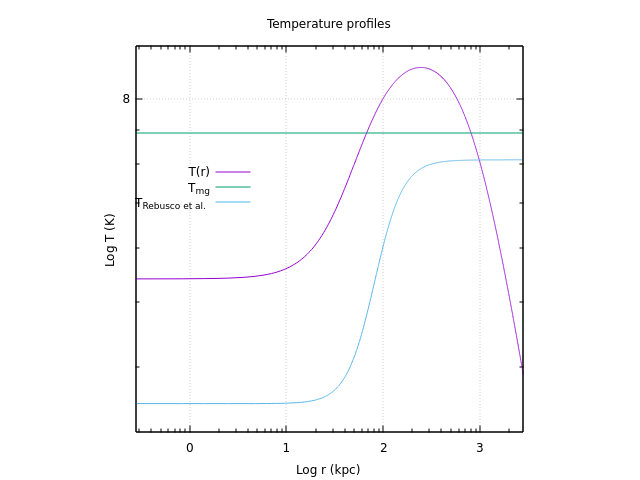
\includegraphics[width=\textwidth]{temprofiles.png}
	\end{subfigure}
	\begin{subfigure}{0.49\textwidth}
		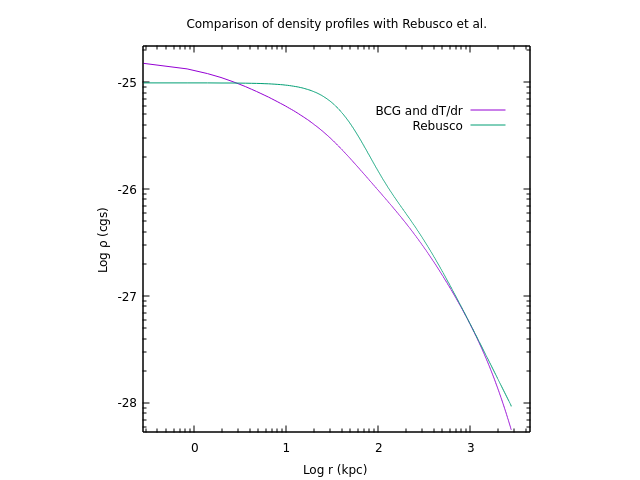
\includegraphics[width=\textwidth]{rebrho.png}
	\end{subfigure}
	\caption{On the left: the two gas temperature profiles adopted in the simulation. The purple curve represents the one given by \eqref{Tprof}, while the green line is the isothermal one. The light blue curve is a variable profile contained in \cite{rebusco}.
	On the right: the comparison between the density profile for the non isothermal model (purple curve) and the one contained in the aformentioned article }
	\label{fig:tempprof}
\end{figure}
FIg.\ref{fig:tempprof} shows both the adopted temperature profiles and the density profile obtained in the non-isothermal model compared to the temperature and density profile used in \cite{rebusco}, which are based on the deprojected $XMM-Newton$ data and are described by:
\begin{equation}
	T(r)=7\frac{1+(r/71)^{3}}{2.3+(r/71)^{3}}\text{keV},
\end{equation}
\begin{equation}
	\rho (r)=1.937\times 10^{-24}\left\{\frac{4.6\times 10^{-2}}{[1+(r/57)^{2}]^{1.8}}+\frac{4.8\times 10^{-3}}{[1+(r/200)^{2}]^{0.87}}\right\}\text{g/cm}^{3}.
\end{equation}
In both formulas the $r $ is in kpc. With that being said, the differences between in the mass profiles for the two cases where we consider the presence of the BCG come from the fact that the variable temperature profile is below the constant one below $\sim 60$ and beyond
$\sim 800$ kpc, which means that the gas is colder than the isothermal model and has thus a higher density and mass.

\section{The diffusion of Fe in the ICM}
\subsection{Physical model}

In the second part of the project we study the diffusion of iron in the ICM. Basically, the idea is that the ICM has been enriched by stars (mostly SNIa explosions but also stellar winds) to a level comparable to the ISM in the Milky Way. This means we observe mostly iron, which can be used as our metal tracer.
The Fe abundance ranges from $0.3$ to $0.5 Z_{Fe,\odot}$, where $Z_{Fe,\odot}=0.0018$.
What we want to find is not only the origin and the amount of metals, but also their spatial distributions. Peaked abundance profiles are a characteristic feature of clusters with cool cores, and abundance peaks are probably associated with with BCGs (see \cite{rebusco}), in which SNIa explode, injecting energy ($\sim 10^{51}$ erg each) and metals, especially iron ($\sim 0.7$ M$_{\odot}$ each).
However, the width of the peaks is much broader than the BCG light distribution (see \cite[text]{grandi}), suggesting that there is a mechanism that is transporting the metals originated from within the BCG.\\ 
We assume that this process can be treated as diffusive, and it's produced by stochastic gas motions. Under the assumption of spherical symmetry, we have that the iron density $\rho_{Fe}$ obeys the following diffusion equation:
\begin{equation} \label{diffeq}
	\pdv{\rho_{Fe}}{t}=\frac{1}{1.4}\frac{1}{r^{2}}\pdv{(r^{2}D\rho_{g}\pdv{Z_{Fe}}{r})}{r}+S_{Fe}(r,t), \quad \text{with}\quad Z_{Fe}=1.4\frac{\rho_{Fe}}{\rho_{g}}
\end{equation} 
where $S_{Fe}(r,t)$ is the source term due to the iron injection from the central galaxy, and $D$ is the diffusion coefficient, which is of the order of $D\approx v_{t}l_{t}$ with $v_{t}$ being the typical turbolent velocity and $l_{t}$ the typical turbolent length-scale. Another useful quantity is the timescale for diffusion over a distance $L$: $\tau_{diff}\sim L^{2}/D$.\\
As previously stated, the metals are injected in the ICM by mainly two objects: SNIa, which explode at a rate proportional to the stellar density (at least locally), which is described
by \eqref{Hern}, and stellar winds. This latter source is proportional to the stellar density $\rho_{*}(r)=\frac{M_{BCG}}{2\pi}\frac{a}{r}\frac{1}{(r+a)^{3}}$.\\
Taking them into consideration, the formula for the source term as a function of time and distance from the centre is:
\begin{equation} \label{source}
		S_{Fe}(r,t)=\rho_{*}(r)\left[\alpha_{*}(t)\frac{Z_{Fe,*}(r)}{1.4}+\alpha_{Ia}(t)\frac{M_{Fe,Ia}}{M_{Ia}}\right],
\end{equation}
where $Z_{Fe,*}$ is the stellar Fe abundance profile, $M_{Fe,Ia}\approx 0.74$ M$_\odot$ and $M_{Ia}\approx 1.4$ M$_\odot$ are respectively the Fe and the total mass ejected by a SNIa explosion, while 
$\alpha_{*}$ and $\alpha_{Ia}$ are the specific mass return rate for the stellar winds and SNIa respectively, and are defined as follows:
\begin{equation}\label{rates}
	\begin{cases}
		\alpha_{*}(t)=4.7\times 10^{-20}(\frac{t}{t_{now}})^{-1.26}\\
		\alpha_{Ia}(t)=5.91\times 10^{-21} SNu(t), \quad \text{with}\quad SNu(t)=SNu(t_{now})(\frac{t}{t_{now}})^{-s}
	\end{cases}
\end{equation}
where $t_{now}$ is the current cosmic time ($\approx 13.7$ Gyr), $s\sim 1.1$, and $SNu(t_{now})$ is the number of SNIa per $10^{10}$ L$_{B,\odot}$ per century, for which the observational estimates for elliptical galaxies (BCG in particular) are still quite uncertain, with values in the range $[0.05-0.5]$.\\

\subsection{The simulation}
The grids we adopt here are the same as the ones in the first part, with $Z_{Fe}$ centered on the second one. In order to transform \eqref{diffeq} from a PDE to a FDE we used the Forward-Time Centered Space (FTCS) method, due to the fact that diffusion is isotropic.
Denoting as $t^{n}$ the value of time at the $n$-th iteration, and assuming a constant $D$ and no change in time for $\rho_{g}(r)$, at a generic point ($r_{j+1/2},t^{n}$) the equation for the diffusion term reads as:
\begin{equation}\label{fdediff}
	\frac{\rho_{Fe,j+1/2}^{n+1}-\rho_{Fe,j+1/2}^{n}}{t^{n+1}-t^{n}}=\frac{1}{1.4}\frac{f_{j+1}^{n}-f_{j}^{n}}{(r_{j+1}^{3}-r_{j}^{3})/3},
\end{equation}
where for a generic $f_{j}^{n}$ we have:
\begin{equation}\label{fnj}
	f_{j}^{n}=r_{j}^{2}D\rho_{g,j}(\pdv{Z_{Fe}}{r})^{n}_{j}=r_{j}^{2}D\rho_{g,j}\frac{Z_{Fe,j+1/2}^{n}-Z^{n}_{Fe,j-1/2}}{r_{j+1/2}-r_{j-1/2}},\quad \text{with} \quad \rho_{g,j}=\frac{1}{2}(\rho_{g,j+1/2}+\rho_{g,j-1/2}).
\end{equation}
As for the source term, there are no derivatives present so from a numerical point of view its treatment is fairly easy, with $S_{Fe}(r_{j+1/2},t^{n})$ being simply a function evaluated at that specific point.\\
The time integration requires two boundary conditions at the two extremes of the grid: $\rho_{Fe}(1)=\rho_{Fe}(2)$ and $\rho_{Fe}(j_{max})=\rho_{Fe}(j_{max}-1)$.
Another aspect to keep in mind is that the choice for the timestep is constrained. According to the Von Neumann stability analysis for the FTCS method, we have that the following inequality must hold for this method to be stable:
\begin{equation}\label{stability}
	\Delta t\le \frac{(\Delta r)^{2}}{2D}.
\end{equation}
In our case we have assumed that neither $D$ nor $\Delta r$ change with time, so we only need to calculate $\Delta t $ once, but since in the general case this isn't true we decided to add an array with the values of $D_{j}$ at each $r{j}$ and then we computed $\Delta t $ for each time cycle as:
\begin{equation}
	\Delta t=C\min_{j}\left\{\frac{(r_{j+1/2}-r_{j-1/2})^{2}}{2D_{j}}\right\},\quad \text{with} \quad C=0.4.
\end{equation}
The last thing we need to complete our setup is the initial abundance of iron. We simulated three different scenarios:
\begin{itemize}
	\item the initial Fe abundance is the one observed in Perseus (see \cite{rebusco}), which, rescaled by a factor $1.4$, is:
			\begin{equation}\label{Feab}
				Z_{Fe,obs}(r)=0.42\frac{2.2+(\frac{r}{80 kpc})^{3}}{1+(\frac{r}{80 kpc})^{3}}Z_{Fe,\odot},
			\end{equation}
			from which we then subtract the constant background value $Z_{Fe,b}=0.4Z_{Fe,\odot}$ (in order to isolate the Fe-peak produced by the SNIa), and we evolve in presence of only diffusion;
	\item  $Z_{Fe}=0$ everywhere and we consider only the source term;
	\item  $Z_{Fe}=0$ everywhere, but with both source and diffusion present.
\end{itemize}
We choose as our gas density profile the one corresponding to the non-isothermal model of the previous part. It's also important to notice that we consider the $Z_{Fe,*}$ to be constant and equal to the solar one in the source term.\\
Considering $v_{t}=260 km/s$ and $l_{t}=15kpc$ and a multiplicative constant $C=0.11$ our standard value for the diffusion coefficient is $D=1.32\times 10^{29}$cm$^{2}$/s, however we do change it in some simulations.
\subsection{Results and discussion}
For all the different scenarios, we run the simulation for three different integration times: $t_{1}=1 $ Gyr, $t_{2}=2$ Gyr, and $t_{3}=5$ Gyr. Fig. \ref{fig:Zdiffonly}, \ref{fig:Zsourceonly}, and \ref{fig:Zdiffsource} show the numerical metallicity profiles determined for the diffusion-only, source-only and diffusion+source models for the three integration times.
\begin{figure} [H]
	\centering
	\begin{subfigure}{0.49\textwidth}
		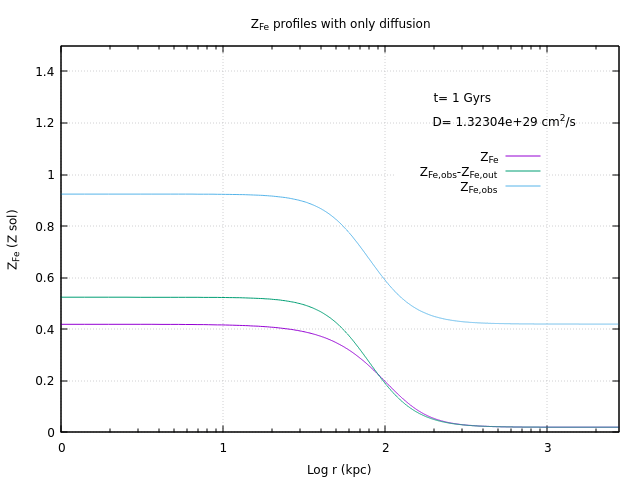
\includegraphics[width=0.9\linewidth]{Z_diff_1.png}
	\end{subfigure}
	\begin{subfigure}{0.49\textwidth}
		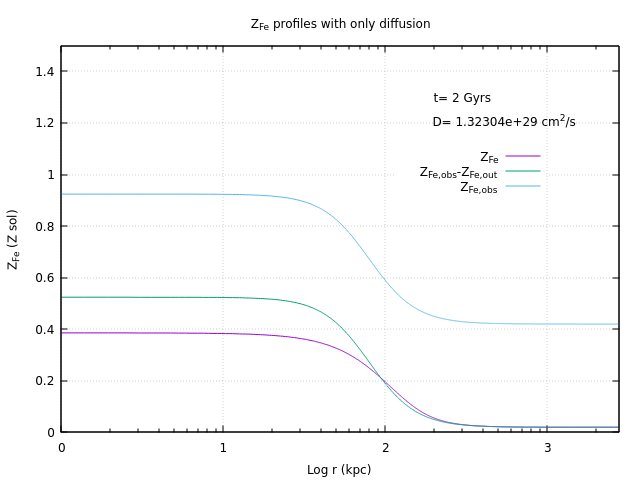
\includegraphics[width=0.9\linewidth]{Z_diff_2.png}
	\end{subfigure}
	\begin{subfigure}{0.49\textwidth}
		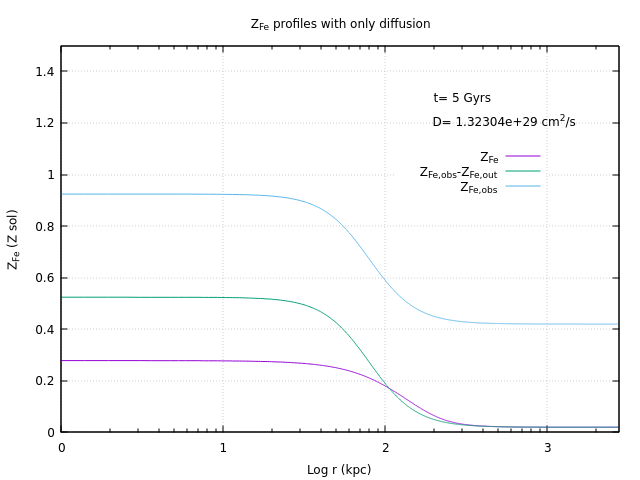
\includegraphics[width=0.9\linewidth]{Z_diff_5.png}
	\end{subfigure}
	\caption{\textit{From left to right and from top to bottom:} Fe metallicity profiles evolved in the case with only diffusion, respectively for $t_{1}=1 $ Gyr, $t_{2}=2$ Gyr, and $t_{3}=5$ Gyr. The light blue curve shows the numerical integration of \eqref{Feab}, the green curve is the same but with the subtraction of the background metallicity and the purple curve is the final profile.}
	\label{fig:Zdiffonly}
\end{figure}
For the diffusion-only model we also check the values of the mass within $100$ kpc as well as the total one in the whole grid, in order to check if it's conserved. For the former, the results at the three different times were $M_{Fe}(r<100\text{kpc},t_{1})=3.31\times10^{8}$M$_{\odot}$,$M_{Fe}(r<100\text{kpc},t_{2})=3.16\times10^{8}$M$_{\odot}$,
 and $M_{Fe}(r<100\text{kpc},t_{3})=2.56\times10^{8}$M$_{\odot}$, while the latter is the same for all times, with $M_{Fe,tot}=7.08\times10^{9}$M$_{\odot}$. 
 We also estimate the diffusion time by defining it as the time needed for the mass contained in a radius $L=80$kpc to be reduced by a factor 2: considering as diffusion coefficient the usual value, we get $\tau_{diff}=11.3$Gyr, which is comparable to the one obtained with the formula $\tau_{diff}=L^{2}/D=14.6$ Gyr. 
\begin{figure}[H]
	\begin{subfigure}{0.50\textwidth}
		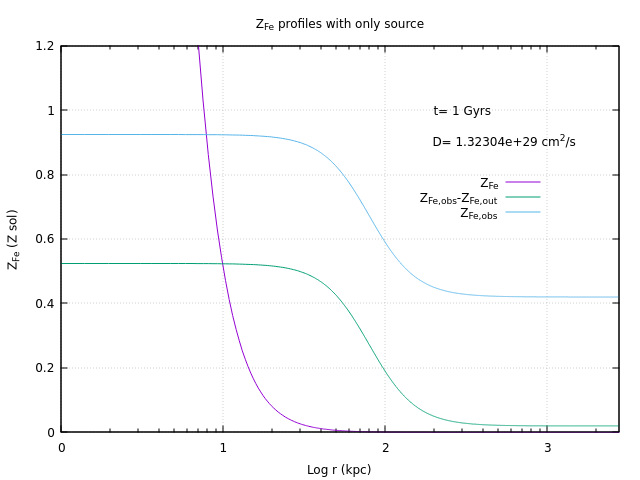
\includegraphics[width=0.9\linewidth]{Z_source_1.png}
	\end{subfigure}
	\begin{subfigure}{0.49\textwidth}
		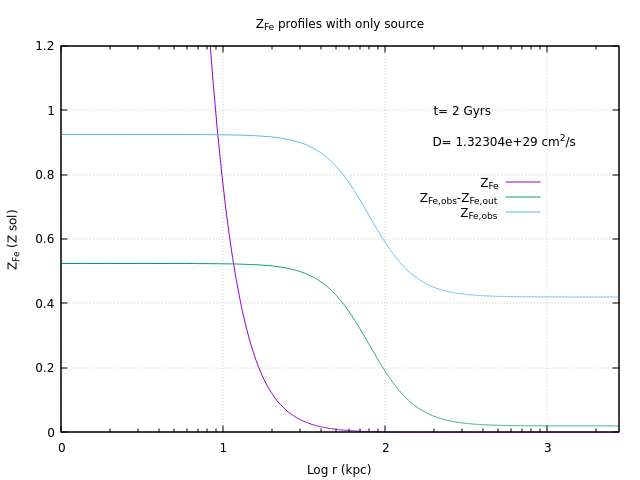
\includegraphics[width=0.9\linewidth]{Z_source_2.png}
	\end{subfigure}
	\begin{subfigure}{0.49\textwidth}
		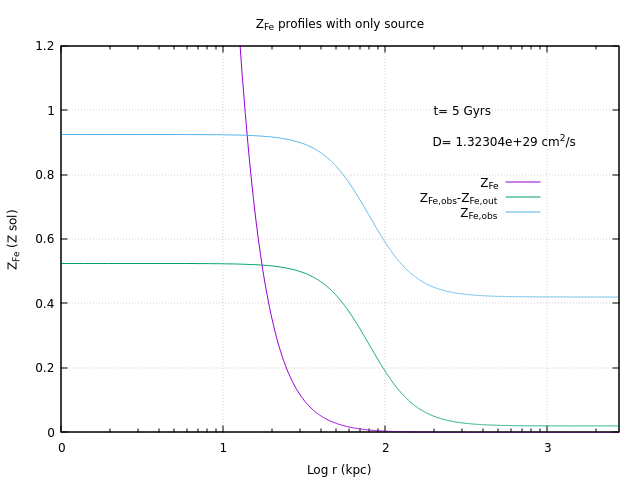
\includegraphics[width=0.9\linewidth]{Z_source_5.png}
	\end{subfigure}
	\begin{subfigure}{0.49\textwidth}
		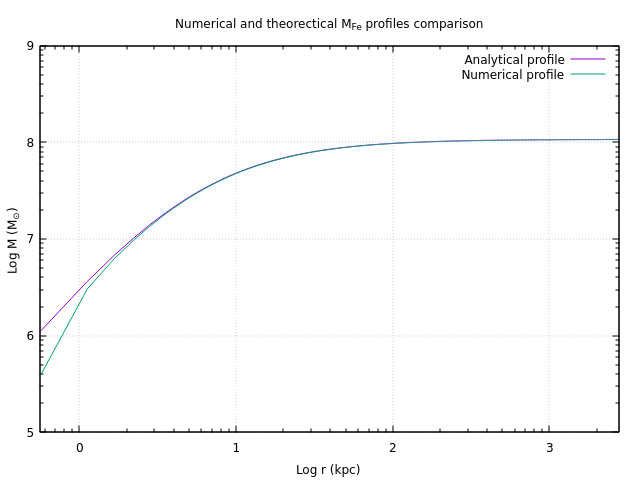
\includegraphics[width=0.9\linewidth]{femass_comparison.png}
	\end{subfigure}
	\caption{\textit{From left to right and from top to bottom:} the first three plots show how Fe metallicity profiles evolved in the case with only source, respectively for $t_{1}=1 $ Gyr, $t_{2}=2$ Gyr, and $t_{3}=5$ Gyr. The light blue curve shows the numerical integration of \eqref{Feab}, the green curve is the same but with the subtraction of the background metallicity and the purple curve is the final profile.
	The last plot shows the comparison between the numerical iron mass profile (green curve) and the analytical one (purple curve) after $5$ Gyr.}
	\label{fig:Zsourceonly}
\end{figure}
For the source-only model, we considered the half-mass radius as a way to determine the size of the Fe-peak, which gave a value of $R_{Fe,1/2}=12.3$ kpc for all three times. We then compare the total Fe masses obtained numerically to the ones obtained by integrating over time and volume the source term; for $t_{1}$ we get $M_{Fe,tot}=1.74\times10^{7}$M$_{\odot}$ and $M_{Fe,tot}^{theo}=1.74\times10^{7}$ m$_{\odot}$, for $t_{2}$ we get $M_{Fe,tot}=3.63\times10^{7}$M$_{7}$ and $M_{Fe,tot}^{theo}=3.65\times 10^{7}$M$_{\odot}$, and for $t_{3}$ we get $M_{Fe,tot}=1.06\times10^{8}$M$_{\odot}$ and $M_{Fe,tot}^{theo}=1.07\times10^{8}$ m$_{\odot}$.
\begin{figure}[H]
	\begin{subfigure}{0.49\textwidth}
		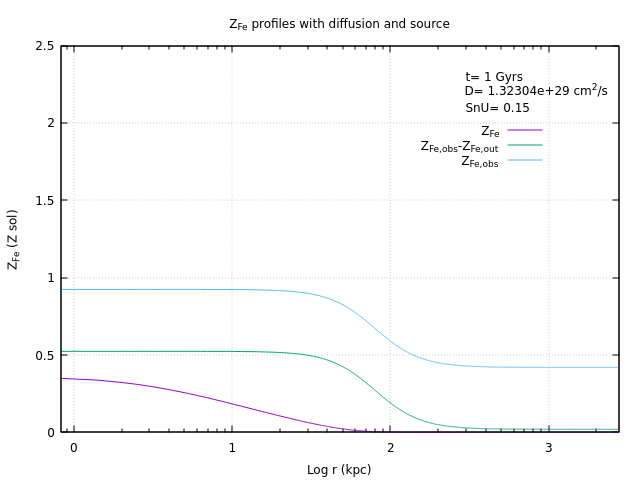
\includegraphics[width=0.9\linewidth]{Z_diffsource_1.png}
	\end{subfigure}
	\begin{subfigure}{0.49\textwidth}
		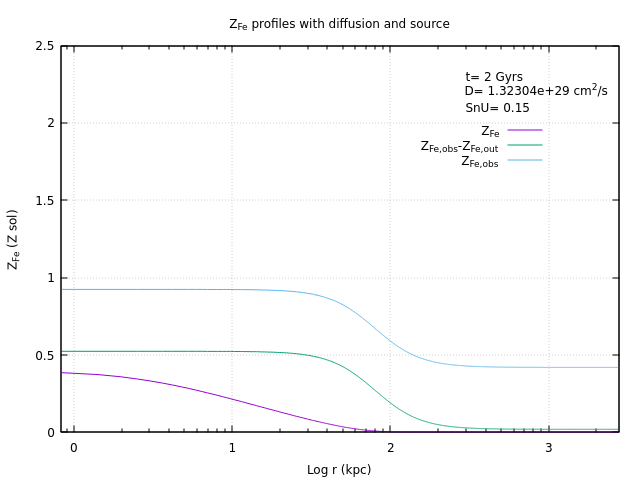
\includegraphics[width=0.9\linewidth]{Z_diffsource_2.png}
	\end{subfigure}
	\begin{subfigure}{0.49\textwidth}
		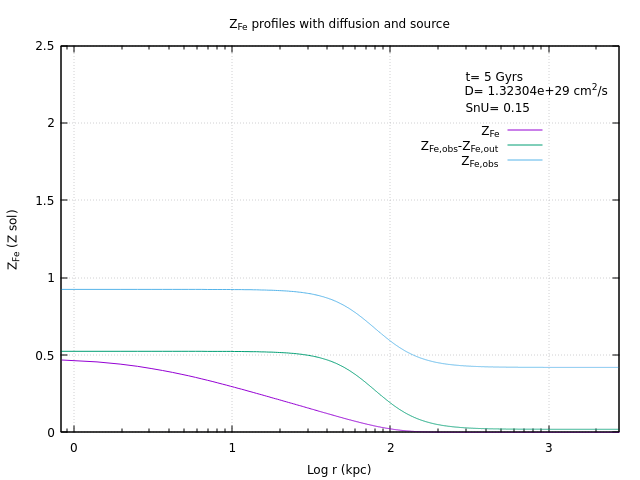
\includegraphics[width=0.9\linewidth]{Z_diffsource_5.png}
	\end{subfigure}
	\begin{subfigure}{0.49\textwidth}
		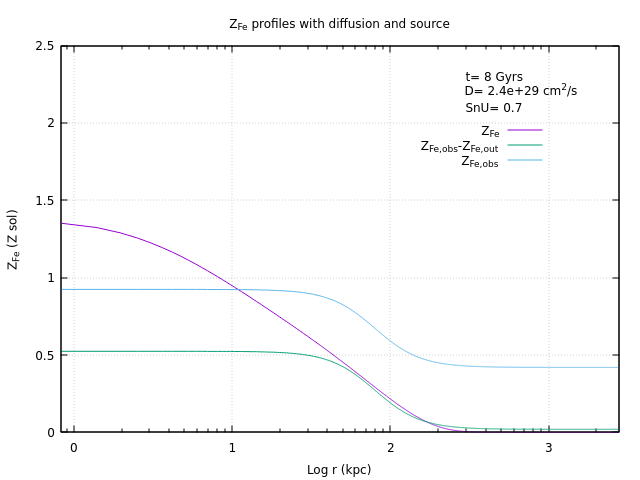
\includegraphics[width=0.9\linewidth]{Z_diffsource_8.png}
	\end{subfigure}
	\caption{\textit{From left to right and from top to bottom:}the first three plots show the Fe metallicity profiles evolved in the presence of both diffusion and source (purple curve), first for $t_{1}=1$Gyr, then for $t_{2}=2$Gyr and lastly for $t_{3}=5$Gyr. The last plot shows the same profile but evolved for $t_{4}=8$ Gyr and with $D=2.4\times 10^{29}$cm$^{2}$/s. For this last plot the value of $SNu(t_{now})=0.7$ has been used.}
	\label{fig:Zdiffsource}
\end{figure}
For the third model, we obtain for the half-mass radii and total Fe masses the following values: $R_{Fe,1/2}(t_{1})=38.6$ kpc, $R_{Fe,1/2}(t_{2})=43.7$ kpc, and $R_{Fe,1/2}(t_{3})=63.9$ kpc,
$M_{Fe,tot}(t_{1})=2.43\times10^{7}$M$_{\odot}$, $M_{Fe,tot}(t_{2})=3.62\times10^{7}$M$_{\odot}$, and $M_{Fe,tot}(t_{3})=1.06\times10^{8}$M$_{\odot}$.
The values of the half-mass radii all exceeds the half-light radius of the BCG ($r_{1/2}=12$ kpc), which means that turbolent diffusion could be the mechanism we need to explain the spreading of Fe outwards. However, from Fig.\ref{fig:Zdiffsource} we can see that the numerical profile is not able to reproduce the observed one. The only plot that has a good agreement with the observations is the fourth one in the region with $r>50$ kpc, where we changed the values of $D$, $SNu(t_{now})$, and the integration time, which was set to $8$ Gyr, so an old cluster.
\section*{Conclusions}
We start from three different initial assumptions to get three different density profile in the hydrostatic equilibrium configuration. We can explain the differences between them with the change in the gravitational field due to the addition of the BCG, which causes a steepening, as well as with the adoption of a gradient in the temperature, which causes the gas to be hotter than the isothermal one in the range between $60$ and $800$ kpc. We then proceed to study the emission of Fe in the ICM and we try to determine what mechanism lies behind it. We determine that turbolence could be the cause and we show that with a diffusion coefficient $D=2.4\times 10^{29}$ cm$^{2}$/s and a value
of $SNu(t_{now})=0.7$, using the model with both diffusion and source, we get that iron is diffused several times above the half-light radius of the BCG, as well as a good agreement with the observed Fe profile.


\begin{thebibliography}{3}
	\bibitem{cimatti}
	A. Cimatti, F. Fraternali, and C. Nipoti. Introduction to Galaxy Formation and Evolution.
From Primordial Gas to Present-Day Galaxies. Cambridge University Press, 2020.
	\bibitem{rebusco}
	P. Rebusco et al. “Impact of stochastic gas motions on galaxy cluster abundance profiles”.
In: Mon. Not. R. Astron. Soc. 359 (2005), pp. 1041–1048. doi: https://doi.org/10.
1111/j.1365-2966.2005.08965.x.
\bibitem{grandi}
S. De Grandi et al. “On the Fe abundance peak formation in cool-core clusters of galaxies:
hints from cluster WARPJ1415.1+3612 at z = 1.03”. In: A\&A 567 (2014). doi: https:
//doi.org/10.1051/0004-6361/201423928.
\end{thebibliography}
\end{document}